%----------------------------------------------------------------------------------------
%	PACKAGES AND OTHER DOCUMENT CONFIGURATIONS
%----------------------------------------------------------------------------------------

\documentclass[paper=a4, fontsize=10pt]{scrartcl} % A4 paper and 11pt font size

\usepackage[T1]{fontenc} % Use 8-bit encoding that has 256 glyphs
\usepackage[english]{babel} % English language/hyphenation

\usepackage{sectsty} % Allows customizing section commands
\allsectionsfont{\centering \normalfont\scshape} % Make all sections centered, the default font and small caps

\usepackage{fancyhdr} % Custom headers and footers
\pagestyle{fancyplain} % Makes all pages in the document conform to the custom headers and footers
\fancyhead{} % No page header - if you want one, create it in the same way as the footers below
\fancyfoot[L]{} % Empty left footer
\fancyfoot[C]{} % Empty center footer
\fancyfoot[R]{\thepage} % Page numbering for right footer
\renewcommand{\headrulewidth}{0pt} % Remove header underlines
\renewcommand{\footrulewidth}{0pt} % Remove footer underlines
\setlength{\headheight}{13.6pt} % Customize the height of the header

\usepackage{amsmath} % Enable number within
\numberwithin{equation}{section} % Number equations within sections (i.e. 1.1, 1.2, 2.1, 2.2 instead of 1, 2, 3, 4)
\numberwithin{figure}{section} % Number figures within sections (i.e. 1.1, 1.2, 2.1, 2.2 instead of 1, 2, 3, 4)
\numberwithin{table}{section} % Number tables within sections (i.e. 1.1, 1.2, 2.1, 2.2 instead of 1, 2, 3, 4)

\usepackage[pdftex]{graphicx} % Enable including png's

\setlength\parindent{0pt} % Removes all indentation from paragraphs - comment this line for an assignment with lots of text

%----------------------------------------------------------------------------------------
%	TITLE SECTION
%----------------------------------------------------------------------------------------

\newcommand{\horrule}[1]{\rule{\linewidth}{#1}} % Create horizontal rule command with 1 argument of height

\title{	

\includegraphics[width=2.3272in,height=1.0417in]{template-img1.png}\\
\normalfont \normalsize 
E-communicatie\\
Toegepaste Informatica \\
\textsc{KHLeuven} \\ [25pt] % Your university, school and/or department name(s)
\horrule{0.5pt} \\[0.4cm] % Thin top horizontal rule
\huge Steroids for your development environment\\ % The assignment title
\small A compilation of techniques and tools to improve your work-space. % Optional subtitle
\horrule{2pt} \\[0.5cm] % Thick bottom horizontal rule
}

\author{Kevin Jossart} % Your name

\date{\normalsize\today} % Today's date or a custom date

\begin{document}
\begin{titlepage}
\maketitle % Print the title
\end{titlepage}

%----------------------------------------------------------------------------------------
%   Table of Content
%----------------------------------------------------------------------------------------

\tableofcontents % Print the table of contents
\newpage % On its own page

%----------------------------------------------------------------------------------------
%	INTRODUCTION
%----------------------------------------------------------------------------------------

\section{Introduction.}

In this article I will try to convince you, being a developer, why you should not just
be happy with the defaults when it comes to your development environment. If
you never figure out how to use your computer well you will never become a master that everyone looks up to.
\newline
\newline
Think about it like a professional cyclist would, he might be able to become a
great cyclist by just training a lot, but having the right bike made to fit his
body will certainly give him that extra edge he needs to distinguish himself
from the other cyclists.
Like a cyclist, developers have a set of tools they need to be able to
do their job (a.k.a the bike). And like a cyclist you will want the perfect one.
In the next following pages I will discus the most important
aspects of a developer environment, the things you will most likely want and
the things you will most likely not want. Of course some of these things might
be a bit subjective so I can't guarantee that you will always agree with me. If
not I will do my best to convince you otherwise!
\newline
\newline
Everything discussed in this document will have a link to it's homepage or
Wikipedia. I hope, if you take the effort of reading this, you will also take
the effort of following the included links in this document. The websites of
these software  will be much more thorough than what I could ever
hope to write in an article like this. 
\newline
Everything in this article will also be language agnostic, so you don't need to
be using a specific language for this or that tool. I am very adamant about
this, I feel that having a different tool set for each language is a
horrible thing and really makes progressing and learning 10 to a 100 times
harder than it could be. For example, I can use vim to type in this document in
.TeX format, I could create a java program, write a script, edit some configuration
files all in the same environment I am so used to working in. Using a
traditional approach I would have to install a different piece of software for
each of these tasks. Using Vim allows me to just learn one text editor and learn it properly and not be hindered by the
fact that I need a different set of software for each task I have in front of
me! 

\subsection{Why did I choose this  topic?}

Ever since I started my education in Applied Computer Science I ran into the
feeling that the thing I was doing could be done faster, with less effort. I
tried to be as lazy as possible and let my computer do the hard work for me.
For some time now I have been actively researching techniques to make my life
easier. I currently also maintain a public repository that allows people who
want to use vim ( a very famous UNIX text editor ), but do not want to be bothered with all the details of setting
it up or who switch computers often, to do this configuration
automatically. Seeing as I have done all this research in the recent years I
hope that I can bring some interesting things to your knowledge and be able to
write an interesting article.

%----------------------------------------------------------------------------------------
%  Operating Systems
%----------------------------------------------------------------------------------------

\section{Choosing an Operating System.}
This is the first choice you will have to make when setting up your development
environment, and sadly the one that probably get's neglected the most because of
pure laziness. It would be easy for me to just tell you which OS you should
choose, I tend to be quite biased, and be done with it! But I will not do that and explain the pros and
cons of each Operating System.

\subsection{Windows}
Windows is a great operating system, it has support for almost any software on
the planet, you can play games with it, it is easy and installing windows is a
breeze. What it is not useful for, sadly enough, is development. Why is that you
ask? It does not have a central software repository, having to manually fetch
software from the internet and install it yourself is bad. It lacks a proper terminal and server support
making deploying and testing unnecessarily hard and most of the tools you'd
love to use in a terminal are not available, forcing you to integrate it into
an IDE even if you would prefer to use it separately. I honestly suggest, if you
are not a windows only developer(I'm sorry for you), to look a bit farther than
your nose is and find a whole plethora of operating systems that would love to
become your new daily driver. I am by no means implying that you can't use
windows anymore, as I said it is great at what it does, but  developers are not
their target audience which cripples them in various ways.

\subsection{GNU/Linux Derivatives}
So you have decided to learn and pick up a Linux distribution for your
Development Environment? Good choice! You and your employer will be quite happy
with the choice. Depending on your hardware or the distribution of your choice
you might have to put some real work in it to have a fully operational Operating
System. But this work comes with an advantage! Choices! You can decide what
runs on your computer, from the most trivial component to the kernel itself!
Using a Linux desktop you have access to the following pro's compared to
Windows:

			\begin{itemize}
                \item A central software repository,
which is an incredibly easy way to safely get all the software you need on your
computer;
			    \item Most Github applications are tailored for Linux
                    distributions first;
                \item Linux distributions have a proper terminal;
                \item Deploying servers, installing libraries, compiling
                    software is all done easily from the terminal.
			\end{itemize}

All these benefits will greatly help you create better software with less
effort. Using a terminal and managing all of these
great benefits is not easy though, but make the effort to learn and you will thank
yourself in the end! 
\subsubsection{Fedora\cite{fedora}}
Why am I only taking a deeper look at Fedora you might ask? Well I've used it
for 4 years now and I just feel very strongly about what Fedora does right.
They are also the only flavor that actively promote the fact that they are
made for DEVELOPERS and not normal users.
\newline
\newline
Fedora is for those that love a steeper, more motivating, learning curve. It's
easy to use, but it comes pretty minimal out of the box, not really minimal,
but far less complete with pre-installed application software than the previous
two. Fedora is also very strict in refusing non-free packages, and has very
strict packaging quality rules, so for instance, Chromium is not allowed in the
official Fedora repos. So for Google Chromium lovers, you'll have to compile
yourselves, use the packages from OpenSUSE\cite{suse}, or just go for OpenSUSE altogether.
\newline
\newline
Fc21 is a technical bleeding edge distribution, the technology under the hood goes a
step further than any other distribution. You'll find things like alternative
compilers, full 3D printer integration, the best Docker\cite{docker} and
Sandstorm\cite{sandstorm}
integration (and on the Fedora Cloud version the Atomic server functionality
for those that really want to taste the future of software development and
marketing), the latest version of your favorite text editor, all the latest
development, scientific and computational tools, the latest kernels, the latest filesystem features, etc...
\newline
\newline
It's a distribution for engineers, scientists and developers that are really into
their game, and know what they want, but at the same time, it's also a very
accessible learning platform for people that want to elevate their skills and
are really into stuff like that. It's also the community distribution that is closest
to the reference enterprise GNU/Linux distribution, Red Hat Enterprise Linux.
Together with SUSE (SLES)\cite{suse}, RedHat (RHEL)\cite{redhat} is the distribution that pretty much makes
the world turn around. These distributions, called RPM-distributions because they use the
"RedHat Package Management" format, are the primary tool that enterprises and
organizations use to shape the future of technology and the world. Fedora is
also the only community distribution (besides AOSP 5 Lollipop that is, but that's not
a GNU/Linux distribution) that comes out of the box with SELinux working as it
should. SELinux\cite{selinux} is the most advanced mandatory access control system that
exists for the moment, and that means that the users can benefit from quite a
substantial extra security layer on their systems.
\newline
\newline
Does all of this good stuff make you want to learn more about fedora? The link
to it's homepage is in the references so go ahead and download an ISO and try
it out yourself. 

\subsection{OSX}
OSX is great, it has most of the benefits of a Linux distribution and is still
as 'easy' as a windows installation. If you are not too adventurous, got cash
to blow, want to use it as a step to Linux, or just want to get started quickly
it is a great choice. Buying a macbook is expensive though and you might not
always be able to choose the hardware or software you need or want... So think carefully
before committing to an apple product. Other than that, with the right amount
of love, OSX can be a great development environment, with a great functional
terminal and good software choices. 

\subsection{OpenBSD\cite{openbsd} and FreeBSD\cite{freebsd}}
If you are into networking, security or have some personal issues with
GNU/Linux but still want to run a similar kind of free system, *BSD systems are
a great choice. OpenBSD\cite{openbsd} and FreeBSD\cite{freebsd} are both interesting
Operating Systems with a lot to offer in terms of great
networking/security/firewalling software. Their only downside at the moment is
because they are shamefully the least popular Operating Systems in this list,
their hardware support can sometimes be a bit lacking. *BSD's focus is very much security, and they have made some very big contributions to
security on the internet, see OpenSSH for a good example, but lately they
started making some great leaps to their desktop experience with more
applications and hardware running natively on *BSD computers than ever before. But my description
here is very much lacking, so please check out their respective websites. This article\cite{whatisbsd} is very
helpful in getting to know *BSD systems and learn about the differences with a
GNU/Linux system. 
%----------------------------------------------------------------------------------------
%  Text Editors 
%----------------------------------------------------------------------------------------

\section{The text editor debate!}
\subsection{My two cents about IDE's}
I don't like them. I wish I could just type this and be done with it. But in an
effort to not be unfair, I will give a reason as to why I don't like them and also
point out the things they do well. My main gripe with IDE's is that they are
always too language specific and if you want to be able to use them for an other language
you need to install a complete overhaul plugin that often breaks and/or crashes
your IDE. This way you end up having to
learn a new IDE for every language you pick up or maybe even for every new
project you have to work on. Because of this you never get to learn the details
and settings of your IDE(If they haven't been hidden behind several windows, subtabs,
dropdowns, etc..).
\newline
\newline
My next problem with them is that for all the good things IDEs have brought us (smart auto-completion, nice
visual debuggers, semantic analysis of the source code, etc) they have totally
forgot about the most crucial part of software development - it's mostly about
editing text. And all the IDEs I've used have extremely poor text editing
capabilities compared to likes of Emacs and vim. A very trivial example is the
fact that most IDEs don't even have key bindings optimized for touch typing -
they require you to move your hands often from the home row (such a waste) and
have mouse-centric UIs.  A programmer's editor might not have all the fancy
bells and whistles - but it has the thing that matters (should matter) the most
- a decent editing experience.

\subsection{Text editors}
And because of my issues with IDE's we start looking at Text editors. I will
talk about the 3 most interesting ones at the moment. If you are
not satisfied with either of these you can find some more interesting stuff
here, \newline\emph{www.github.com/showcases/text-editors}.\newline 
While vim and Emacs both might seem a little bit empty and ugly straight out of
the box, they are infinitely extensible, completely configurable and really
really good. The learning curve on both of these editors is quite high and it
may take some time to get your initial setup done but let me tell you it is
worth it! The manuals, wikis and extensions are vast and there is a great community around both of these text editors, this means
that you can ask questions on stackoverflow if you need to. My presentation of
the different text editors will be quite brief, not only because there are so
many great articles already that are only about that article but also because I
do not want to needlesly make this article even longer. I will refer to good
article's concerning each editor. Now let's get into
the details of these text editors, and see what each of them does to become so
great!
\newline
\newline
\small % Just a small postscript to this paragraph
I am consciously not including Sublime here because it is not free(free beer and freedom). Lime is
an open source alternative to Sublime that I do like. You can find it in the link above.
\normalsize % Return to normal settings
\subsubsection{Vim\cite{vim}}
Vim is probably the most powerful editor ever made. It is also fundamentally
different compared to any other editor. This is because it uses modal editing.
This means that in vim you can't just start typing text. You have to enter
Insert Mode first. The 3 most important modes are Insert Mode, Command Mode and
Selection Mode. Because of this modal editing, Vim is extremely powerful and complex edits are
just a few keystrokes away. Straight out of the box vim is already ready to use but
from my experience most people go quite far in customizing their personal copy.
I myself am a great example\cite{numkilvimconf}. Because everything is a
plugin, you can choose yourself what you need and what you don't need. Someone
has already made a plugin for every possible usecase you can ever imagine!
Because of all these choices and radically different features Vim's learning
curve is quite high, But I really think that learning an editor for a few weeks
is well worth it seeing as you probably will be programming for many years more
to come. If you need more convincing as
to why vim is such a great editor, I propose you read the following
article\cite{whousesvi}.
\subsubsection{Emacs\cite{emacs}}
Emacs is the king of extensions and plugins. Not even vim can come close to
it's vast amount of plugins and it's great support for them. It even got to the
point where people jokingly refer to Emacs as an Operating System instead of a
text editor. There is a good reason why Emacs and Vim have always been the 2
most popular text editors, they are vastly different but still manage to be
equally powerful. Emacs even has a Vi mode if you want to go really over the
top!
Since I'm not a seasoned Emacs user I propose this article for more convincing
arguments about Emacs.\cite{whousesemacs}
\subsubsection{Atom\cite{atom}}
Atom is a more traditional fully featured text editor which is quite heavily targeting web
developers as their main users. Since a lot of people love web development, I
figured it could have a place in this article as well. Unlike Vim and Emacs,
Atom ships with 90\% of the stuff you could ever want already in the bundle.
Of course there are also a lot of people making extra plugins that you can install on
top of all this. It is also made using
modern web technologies, which is a super cool feature, and really supports
change and extensibility, albeit at the cost of performance. Do you
really feel like you want the power that vim or Emacs would give you, but still
prefer a more traditional feel to your editor then Atom is your best bet!
\newline
\begin{figure}[h]
    \centering
    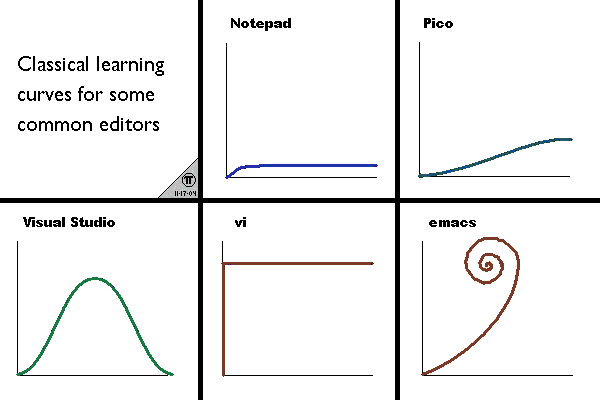
\includegraphics[scale=0.6]{editorlearningcurve.png}
    \caption{Well known joke with a hint of truth!}
\end{figure}

%----------------------------------------------------------------------------------------
%  Customizing your Shell
%----------------------------------------------------------------------------------------
\newpage
\section{Customizing your Shell.}
Most people use Bash\cite{bash} for their shell, there's also some other stuff
like Zsh\cite{zsh}
and Fish\cite{fish} but they are very similar. If you are comfortable with the terminal
emulator you are running your shell in then there isn't that much configuration
you can or need to do to your shell. It's mostly cosmetic and to increase user
friendliness. The most important configuration you can do is to add aliases.
Basically shortcuts to functions or software that you often use yourself. Many of
these configurations can be found on Github under the name DotFiles. These are
all openly available configurations for your shell that you can freely copy and
use yourself. The most interesting ones can be found at this url:\newline
\emph{dotfiles.github.io}\newline
\begin{figure}[h]
    \centering
    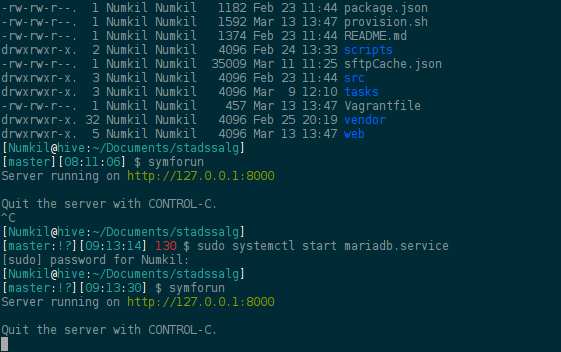
\includegraphics[scale=0.5]{bashexample.png}
    \caption{Interesting example showing cosmetic changes and functionality in Bash}
\end{figure}

%----------------------------------------------------------------------------------------
%  ToolSets
%----------------------------------------------------------------------------------------

\section{A list of indispensable tools.}
All of the tools I will be listing here will be free and are made under some Open
Source or free license. Some web services might charge a monthly subscription for
companies or very heavy users. Single developers or small teams won't run into
this problem however, so I did not exclude them from the list.  I will order
them in their respective categories from most interesting to least interesting in my own opinion.

\subsection{Directory and File management}

\subsubsection{The Silver Searcher\cite{ag}}
The silver searches is just like grep it searches  through your directories and
files for a given regular expression and returns the file and line number of the
places where it could find the regular expression match. The difference with
grep is that is much smarter. It will ignore the files that it already knows
will not contain interesting hits. For example, swap files, cache files,
minified js and css, 3rd party bundle folders etc.. It knows about these files
because of your .gitignore or .hgignore files in a project. If you don't know
about these files already, no worries there's nothing special about them. It's
just a list of directories and files you make inside your project to tell your
versioning system and apparently other software as well that you don't
particularly care about those files for editing purposes. Besides this ignoring
Silver Searches has implemented a whole truckload of optimization's to search
your project fast. If you are interested in learning about how all these
optimization's work you can read quite a lot of blog posts going into the details
of these improvements on the projects home page\cite{ag}. 

\subsubsection{Fuzzy file searching}
Fuzzy file searching is the next incredible tool on my list, it is a
INCREDIBLY fast way to travel through your directories and files! No more going
from directory to directory until you reach your file. No more searching the
right name to click in a folder. You just type some parts of the path+name of the
file and fuzzy file searching would immediately present to you the file you
want. Depending on how unique the name is even 2 letters could be enough to
point fuzzy file searching to the right file.  How does it work: Let's say you
have a file in your project at \emph{/src/folder1/folder2/filename} then you could for
instance type \emph{fo1fil} and let fuzzy file searching point at the file you were
looking for, then you press enter and it opens the file. Depending on the
uniqueness of the name you might only need 2 letters, less unique names may
need up to the whole path of
the file. To demonstrate this type of searching I particularly like this
video\cite{ctrlpvideo}, it's about a VIM plugin called ctrlp that implements
exactly this fuzzy file searching. If you are not a VIM user you do not need to
worry, every major Text Editor or IDE has their own implementation of this
technique.

\subsection{Working in a team}

\subsubsection{Versioning Systems\cite{github}\cite{bitbucket}}
You must have heard about versioning systems already! If not you are probably a
very new programmer or have been living under a rock. These are probably the
most important tool you will ever use to cooperate with your colleagues. They
are used to combine all the edits you and your colleagues have made, track
issues, make versions, branch out, copy and extend other peoples code and so
many more useful operations. The most popular ones at the moment are GitHub\cite{github} and
BitBucket\cite{bitbucket}, they
both use git as the software to control the actual versioning. Git\cite{git} is the most
important and most powerful versioning system out there. It might be a little
tricky at first to learn but it is certainly worth it! Learning about these
versioning systems is not optional, you HAVE to know about them, every company
you will ever work for uses them. And no, dropbox and it's derivatives are not a
valid replacement for a versioning system.

\subsubsection{Docker\cite{docker}}
Docker is for the people who want to be able to deploy their software
without having to do the necessary steps to get a ready system over and over
again. This comes in especially handy when you tend to have lots of people
coming and going in your project and you want them to be able to get started
right away and not have to deal with getting everything ready. The way that it
works is like this, you create a docker container, install everything your
application requires on it, download your source code and optionally build it.
That's it, now whenever you want to deploy your application somewhere you just
make sure they can run dockers and give them the docker. They can now just run
the docker and everything will work exactly the same as it did when you ran the
docker. This way you can make sure the application behaves the same everywhere
you deploy it. This sounds a lot like Virtual Machines doesn't it? It is indeed
almost the same but docker managed to do some Operating System magic to get rid
of most of the extra overhead of running a virtual machine! Interested in how
this works? Docker has a very thorough documentation on it's website and also
an interactive tutorial helping you understand the basics of using docker
containers. You can find the link down in the references. 

\subsubsection{Floobits\cite{floobits}}
Do you know that fancy share editing everyone loves about Google docs where
several people can edit the same file at the same time? Well it has been
possible to share a terminal with colleagues since the 90's using Tmux (A
terminal multiplexer for UNIX-like terminals).
Tmux sharing had it's problems though, you had to open up an ssh port to your
computer and create guest users for your colleagues. Well now Floobits exists,
it implements screen-sharing your terminal in a much safer way. You register at
Floobits with your Github account and Floobits will connect to a proxy where
the files you want to work on 
are temporarily stored and accessible for other people. If you are comfortable
with having public editing 'rooms' then Floobits is a free service. For private
'rooms' and extra services a monthly plan can be purchased. This is maybe
interesting for companies and/or development teams. It exists for
all of the current popular text editors and is also usable from inside a
browser so even if you have colleagues that use an IDE you can work in the same
file together easily. If your code is so sensitive or secret that you can't
trust a third party service, running shh+tmux through a VPN is still a very
powerful combination. 

%----------------------------------------------------------------------------------------
%  Personal effort
%----------------------------------------------------------------------------------------

\section{Conclusion.}
Honestly, this article could have been much longer, and maybe someday it will
be. The world of development is full of interesting people and interesting
software. I hope that my article here has at least got you interested in some
off the cool stuff currently being used by other programmers around the world.
Now that you know about some of the more famous tools you can start looking out
for things yourself. Once you are comfortable with trying new things and
actively staying up to date with all these new tools, you will be able to try
out new things much easier, and seeing yourself improve and become more
efficient will motivate you to do better at your actual work!

\begin{figure}[h]
    \centering
    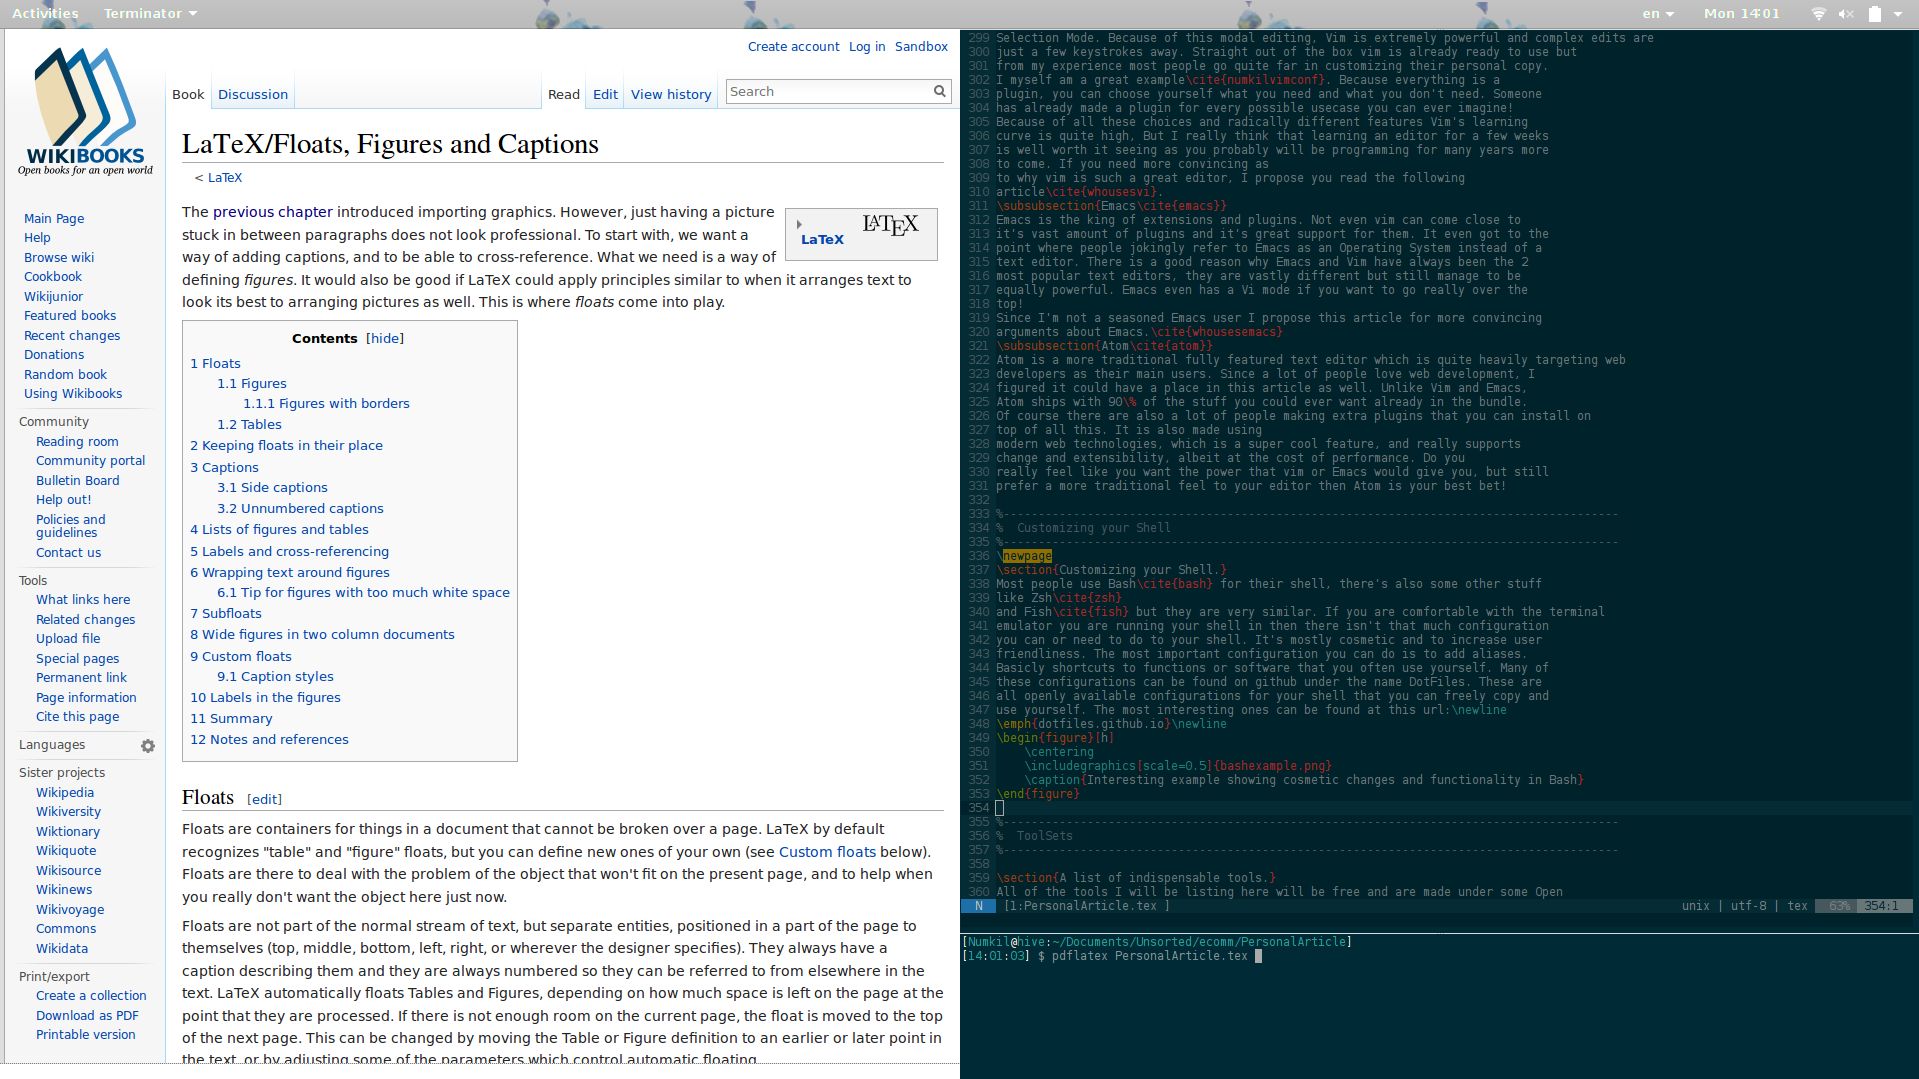
\includegraphics[scale=0.2]{latexprogress.png}
    \caption{This is how I work most of the time.}
\end{figure}

%----------------------------------------------------------------------------------------
%  References 
%----------------------------------------------------------------------------------------

\newpage % I want references on their own page
\begin{thebibliography}{99} % Start references repository here with 99 entries maximum
\bibitem{fedora}
    Fedora Operating System,
    \emph{www.getfedora.org}
\bibitem{suse}
    openSUSE Operating System,
    \emph{www.en.opensuse.org}
\bibitem{redhat}
    RedHat Operating System,
    \emph{www.redhat.com}
\bibitem{teksynfedorasection}
    Forum post used in the fedora section of this article,\newline
    \emph{www.forum.teksyndicate.com/t/gnu-linux-distro-links/72339}
\bibitem{freebsd}
    FreeBSD Operating System,
    \emph{www.freebsd.org}
\bibitem{openbsd}
    OpenBSD Operating System,
    \emph{www.openbsd.org}
\bibitem{whatisbsd}
    Article about the structure and design of *BSD systems,\newline
    \emph{www.over-yonder.net/~fullermd/rants/bsd4linux/01}
\bibitem{vim}
    Vim Text Editor,
    \emph{www.vim.org}
\bibitem{numkilvimconf}
    Numkil Vimconf,
    \emph{www.github.com/numkil/vimconf}
\bibitem{whousesvi}
    Article about using Vi/Vim,
    \emph{www.viemu.com/a-why-vi-vim.html}
\bibitem{emacs}
    Emacs Text Editor,
    \emph{www.gnu.org/software/emacs}
\bibitem{whousesemacs}
    Article about using Emacs,
    \emph{www.batsov.com/articles/2011/11/19/why-emacs}
\bibitem{atom}
    Atom Text Editor,
    \emph{www.atom.io}
\bibitem{bash}
    The most common shell used right now,
    \emph{www.gnu.org/software/bash}
\bibitem{zsh}
    Great alternative to bash,
    \emph{www.zsh.org}
\bibitem{fish}
    Another alternative to bash,
    \emph{www.fishshell.com}
\bibitem{ag}
    The Silver Searcher,
    \emph{www.github.com/ggreer/the\_silver\_searcher}
\bibitem{ctrlpvideo}
    Youtube ShowCase Fuzzy File Searching,\newline
    \emph{www.youtube.com/watch?v=8XGueeQJsrA}
\bibitem{github}
    Github,
    \emph{www.github.com}
\bibitem{bitbucket}
    BitBucket,
    \emph{www.bitbucket.org}
\bibitem{git}
    Git,
    \emph{www.git-scm.com}
\bibitem{docker}
    Docker,
    \emph{www.docker.com}
\bibitem{sandstorm}
    Sandstorm,
    \emph{www.sandstorm.io}
\bibitem{floobits}
    Floobits,
    \emph{www.floobits.com}.
\bibitem{selinux}
    SELinux Mandatory Acces Control,
    \emph{www.selinux.org}
\end{thebibliography}

%------END------------------------------------------------------------------------------

\end{document}
